%author: Pedro Pinto; v2.5; jun 2020
\documentclass[11pt,a4paper]{report}
\usepackage{amsmath}
\usepackage{graphicx}
\usepackage{tabularx}
\usepackage{adjustbox}
%\usepackage[colorinlistoftodos]{todonotes}
\usepackage{csquotes}
\usepackage{comment}
\usepackage{imakeidx}
%tabela
\usepackage{multirow}
\usepackage{xcolor}
\usepackage[margin=3cm]{geometry}
\usepackage[hidelinks]{hyperref}
\usepackage[toc,acronym,nopostdot,nonumberlist]{glossaries}
\usepackage{titling}
\usepackage{tikzpagenodes}
\usepackage[ddmmyyyy]{datetime}
\usepackage{setspace}
\usepackage{indentfirst}

%para definir a localização das tabelas e imagens em modo strict
%\usepackage{placeins}

\usepackage{biblatex}
\addbibresource{ref.bib}
\makeglossaries

%colocar aqui variáveis que serão utilizadas no texto:
\newcommand\kbps{\text{\textit{k}bit/s}}
\doublespacing

\begin{document}

\begin{titlepage}
\begin{tikzpicture}[remember picture,overlay,shift={(current page.center)}]
\node[anchor=center,xshift=0cm,yshift=9.5cm,opacity=0.75]{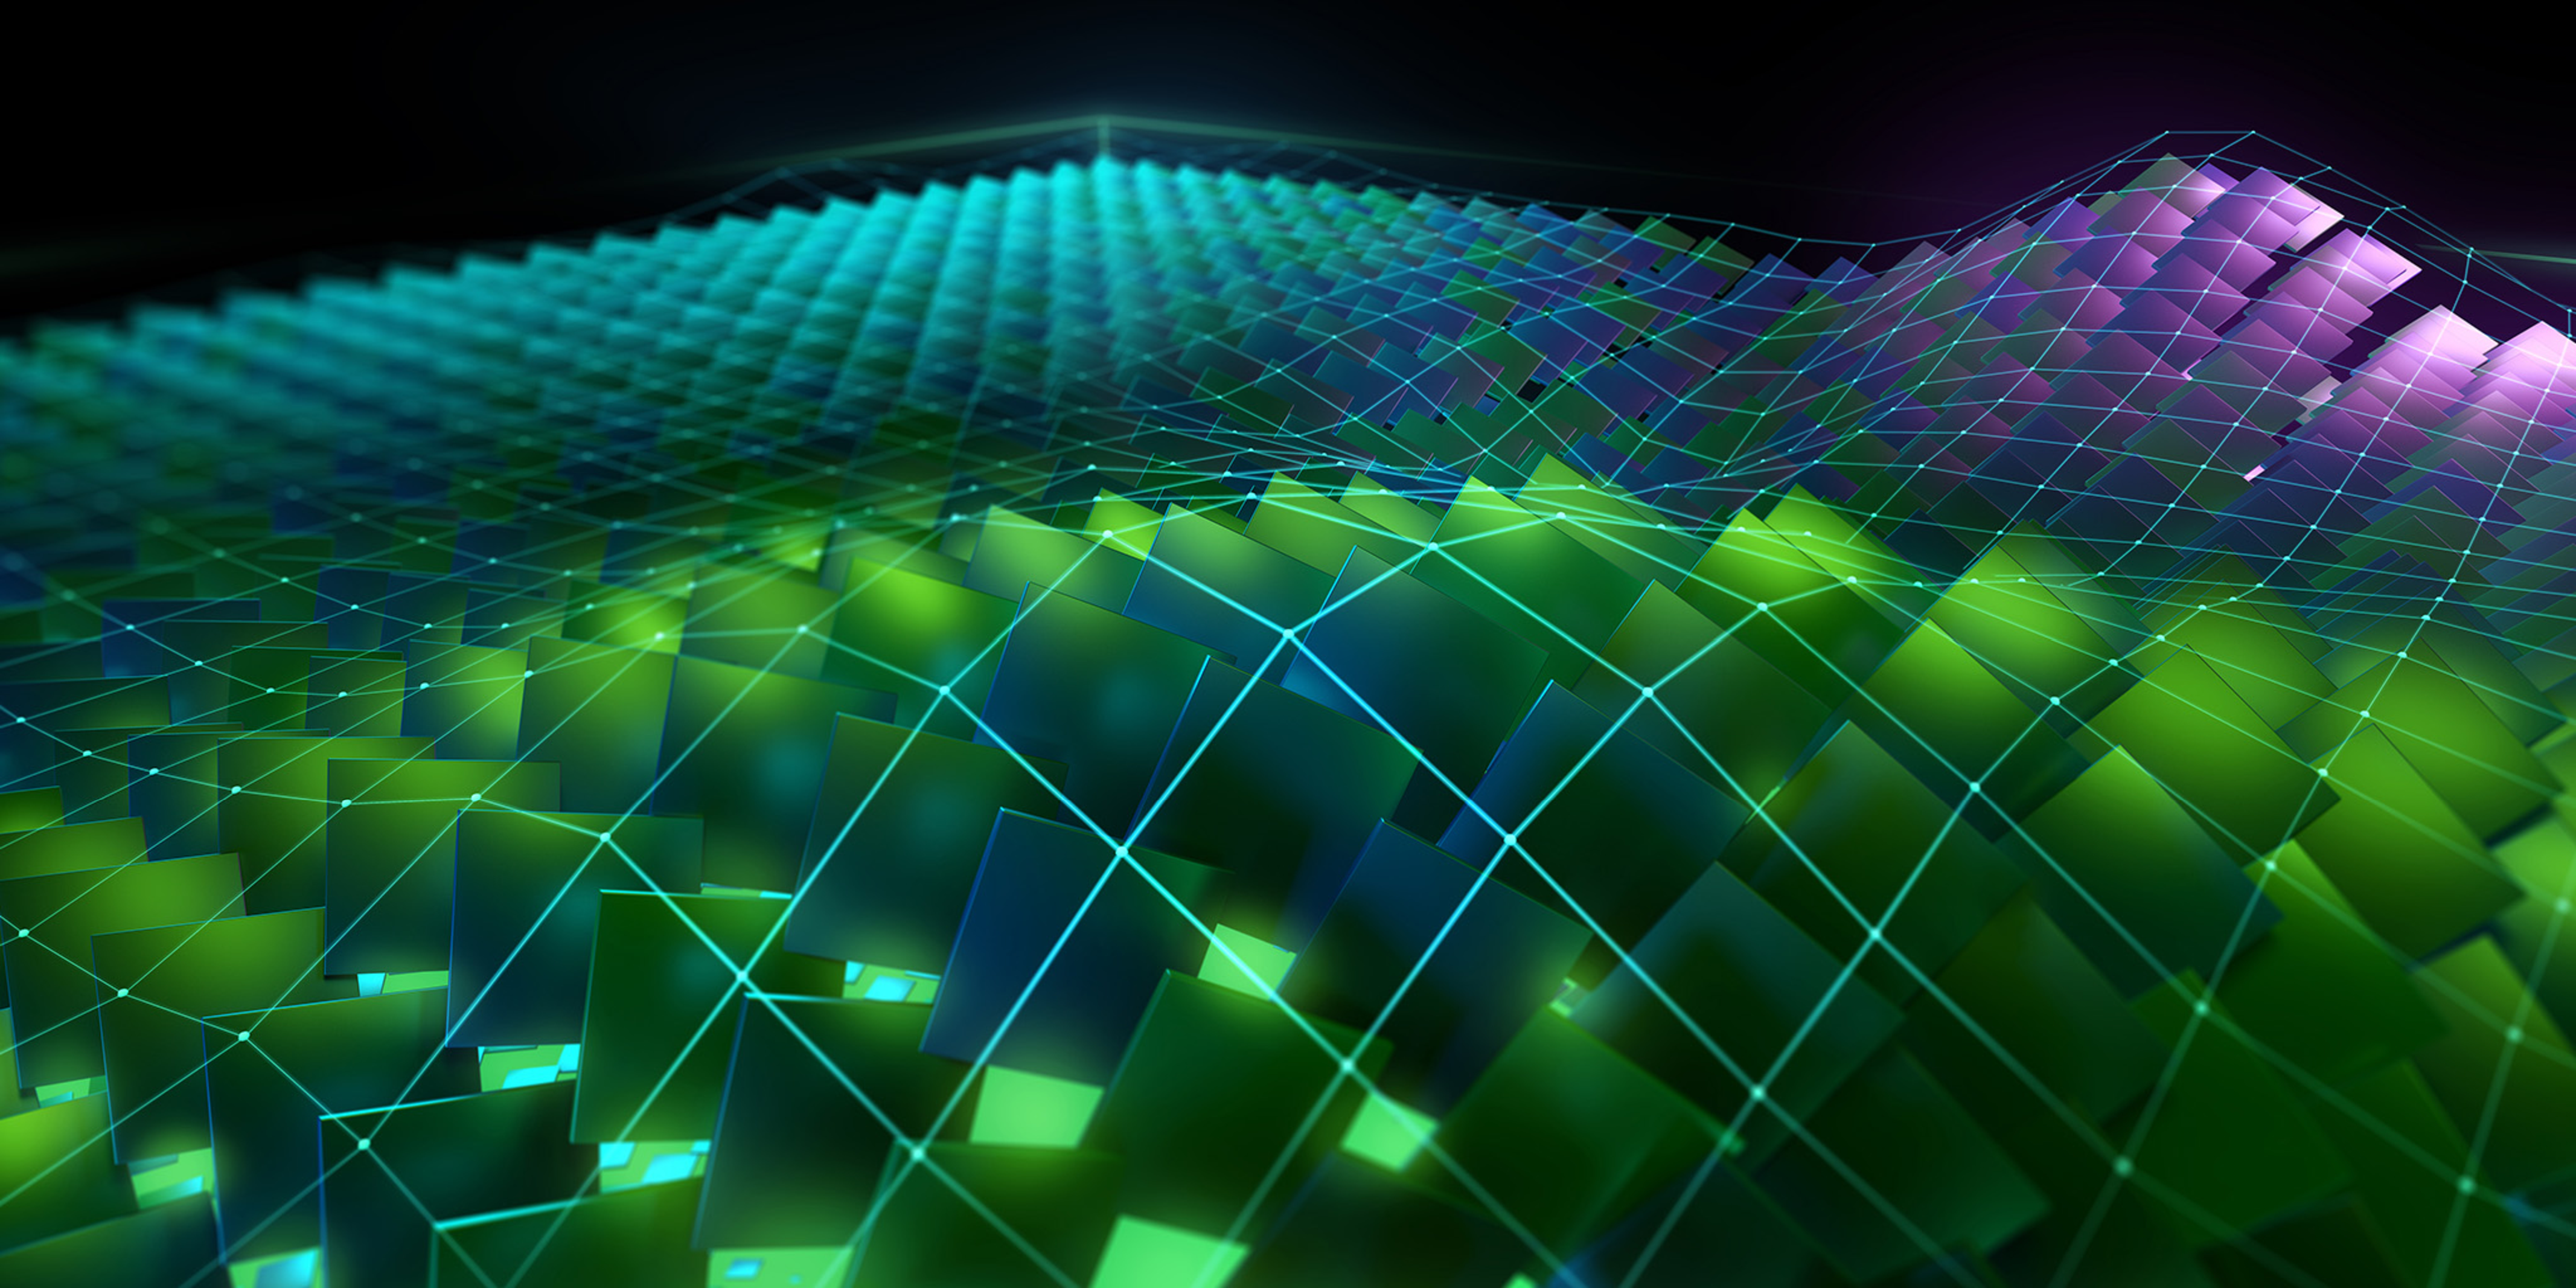
\includegraphics[scale=0.3]{figs/cuda-frontpage.pdf}};
\end{tikzpicture}

\centering
\vspace{10cm}
\huge Classifying CIFAR-10 with Transfer Learning and GPU Acceleration \\
\vspace{3cm}
\large A DD2360 Project\\
%\large a lab assignment report authored by\\
\Large Roderick Karlemstrand\\
\Large KTH Royal Institute of Technology \\

% \large supervised by\\
% %#if Project uncomment
% \large name\\

%#if Internship uncomment following lines
%\large Prof. X (ESTG-IPVC)\\
%\large Name of Company Supervisor (Company X)\\

\vspace{3cm}
%#if Internship uncomment following lines
%\includegraphics[scale=0.35]{figs/ESTG-IPVC.png}

\newdateformat{daymonthyear}{\THEDAY\ \monthname[\THEMONTH], \THEYEAR}
\daymonthyear\today \\
%December, 2019
%\large v2.3
\end{titlepage}

%%%% colocar aqui acrónimos
\newacronym{ersc}{ERSC}{Engenharia de Redes e Sistemas de Computadores}
\newacronym{wn}{WN}{Wireless Network}

%%%%%%%%%%%%%%%%%%%%%%%%%%%%%%%%%%%%%%%%%%%%%%%%%%%%%
\begin{abstract}
%context

%problem

%proposal

%solution

The quick brown fox jumps over the lazy dog. The quick brown fox jumps over the lazy dog. The quick brown fox jumps over the lazy dog. The quick brown fox jumps over the lazy dog. The quick brown fox jumps over the lazy dog. The quick brown fox jumps over the lazy dog.

\end{abstract}


\textbf{Keywords:} word1. word2. word3. word4.

%insert index
\tableofcontents
\glsaddall
\printglossary[type=\acronymtype]
\printglossary[type=main,title={Glossary},toctitle={Glossary}]
%%%%%%%%%%%%%%%%%%%%%%%%%%%%%%%%%%%%%%%%%%%%%%%%%%%%%

\chapter{Introduction}
\label{chap:introduction}

In this Chapter ...test

IMPORTANT:
\begin{itemize}
    \item PLEASE check the file vars.tex: I'm using it in 10\kbps.
    \item Using glossaries for the first time: \gls{wn}
    \item Using glossaries after first time: \gls{wn}
    \item Using glossaries in plural: \glspl{wn}
    \item Using glossaries extended: \glsdesc{wn}
\end{itemize}




This is a way for you to generate tables:

https://www.tablesgenerator.com/

The quick brown fox jumps over the lazy dog. The quick brown fox jumps over the lazy dog. The quick brown fox jumps over the lazy dog. The quick brown fox jumps over the lazy dog. The quick brown fox jumps over the lazy dog. The quick brown fox jumps over the lazy dog.

\section{Context}
\label{sec:context}
%Context
The quick brown fox jumps over the lazy dog. The quick brown fox jumps over the lazy dog. The quick brown fox jumps over the lazy dog. The quick brown fox jumps over the lazy dog. The quick brown fox jumps over the lazy dog. The quick brown fox jumps over the lazy dog.

%context focus
The quick brown fox jumps over the lazy dog. The quick brown fox jumps over the lazy dog. The quick brown fox jumps over the lazy dog. The quick brown fox jumps over the lazy dog. The quick brown fox jumps over the lazy dog. The quick brown fox jumps over the lazy dog.

\section{Problem Statement and Motivation}
\label{sec:motivation}
%problem to solve
The quick brown fox jumps over the lazy dog. The quick brown fox jumps over the lazy dog. The quick brown fox jumps over the lazy dog. The quick brown fox jumps over the lazy dog. The quick brown fox jumps over the lazy dog. The quick brown fox jumps over the lazy dog.

%point the motivation
The motivation of the current project is
The quick brown fox jumps over the lazy dog. The quick brown fox jumps over the lazy dog. The quick brown fox jumps over the lazy dog. The quick brown fox jumps over the lazy dog. The quick brown fox jumps over the lazy dog. The quick brown fox jumps over the lazy dog.

\section{Objectives}
\label{sec:name}
The general objective is to
The quick brown fox jumps over the lazy dog. The quick brown fox jumps over the lazy dog. The quick brown fox jumps over the lazy dog. The quick brown fox jumps over the lazy dog. The quick brown fox jumps over the lazy dog. The quick brown fox jumps over the lazy dog.

\section{Organization}
\label{sec:org}
The quick brown fox jumps over the lazy dog. The quick brown fox jumps over the lazy dog. The quick brown fox jumps over the lazy dog. The quick brown fox jumps over the lazy dog. The quick brown fox jumps over the lazy dog. The quick brown fox jumps over the lazy dog.

\chapter{Title of the chapter}
\label{cap:name1}

The quick brown fox jumps over the lazy dog. The quick brown fox jumps over the lazy dog. The quick brown fox jumps over the lazy dog. The quick brown fox jumps over the lazy dog. The quick brown fox jumps over the lazy dog. The quick brown fox jumps over the lazy dog.

\section{Section 1}
\label{sec:sec1}

The quick brown fox jumps over the lazy dog. The quick brown fox jumps over the lazy dog. The quick brown fox jumps over the lazy dog. The quick brown fox jumps over the lazy dog. The quick brown fox jumps over the lazy dog. The quick brown fox jumps over the lazy dog.

\begin{itemize}
    \item The quick brown fox jumps over the lazy dog. The quick brown fox jumps over the lazy dog. The quick brown fox jumps over the lazy dog. The quick brown fox jumps over the lazy dog. The quick brown fox jumps over the lazy dog. The quick brown fox jumps over the lazy dog.
    \item The quick brown fox jumps over the lazy dog. The quick brown fox jumps over the lazy dog. The quick brown fox jumps over the lazy dog. The quick brown fox jumps over the lazy dog. The quick brown fox jumps over the lazy dog. The quick brown fox jumps over the lazy dog.
\end{itemize}

%%%%%%%%%%%%%%%%%%%%%%%%%%%%%%%%%%%%%%%%%%%%%%%%%%%%%
\chapter{Title of the chapter}
\label{cap:name2}

The quick brown fox jumps over the lazy dog. The quick brown fox jumps over the lazy dog. The quick brown fox jumps over the lazy dog. The quick brown fox jumps over the lazy dog. The quick brown fox jumps over the lazy dog. The quick brown fox jumps over the lazy dog.

\section{Section 2}
\label{sec:sec2}

The quick brown fox jumps over the lazy dog. The quick brown fox jumps over the lazy dog. The quick brown fox jumps over the lazy dog. The quick brown fox jumps over the lazy dog. The quick brown fox jumps over the lazy dog. The quick brown fox jumps over the lazy dog.


\addcontentsline{toc}{chapter}{References}
\printbibliography[title={References}]

\end{document}
